%%%%%%%%%%%%%%%%%%%%%%%%%%%%%%%%%%%%%%%%%%%%%%
% An example of a lab report write-up.
%%%%%%%%%%%%%%%%%%%%%%%%%%%%%%%%%%%%%%%%%%%%%%
% This is a combination of several labs that I have done in the past for
% Computer Engineering, so it is not to be taken literally, but instead used as
% a great starting template for your own lab write up.  When creating this
% template, I tried to keep in mind all of the functions and functionality of
% LaTeX that I spent a lot of time researching and using in my lab reports and
% include them here so that it is fairly easy for students first learning LaTeX
% to jump on in and get immediate results.  However, I do assume that the
% person using this guide has already created at least a "Hello World" PDF
% document using LaTeX (which means it's installed and ready to go).
%
% My preference for developing in LaTeX is to use the LaTeX Plugin for gedit in
% Linux.  There are others for Mac and Windows as well (particularly MikTeX).
% Another excellent plugin is the Calc2LaTeX plugin for the OpenOffice suite.
% It makes it very easy to create a large table very quickly.
%
% Professors have different tastes for how they want the lab write-ups done, so
% check with the section layout for your class and create a template file for
% each class (my recommendation).
%
% Also, there is a list of common commands at the bottom of this document.  Use
% these as a quick reference.  If you'd like more, you can view the "LaTeX Cheat
% Sheet.pdf" included with this template material.
%
% (c) 2009 Derek R. Hildreth <derek@derekhildreth.com> http://www.derekhildreth.com
% This work is licensed under the Creative Commons Attribution-NonCommercial-ShareAlike License. To view a copy of this license, visit http://creativecommons.org/licenses/by-nc-sa/1.0/ or send a letter to Creative Commons, 559 Nathan Abbott Way, Stanford, California 94305, USA.
%%%%%%%%%%%%%%%%%%%%%%%%%%%%%%%%%%%%%%%%%%%%%%

\input kvmacros % For Karnaugh Maps (K-Maps)
\documentclass[UTF8]{ctexart}
\usepackage{graphicx} % For images
\usepackage{float}    % For tables and other floats
\usepackage{verbatim} % For comments and other
\usepackage{amsmath}  % For math
\usepackage{amssymb}  % For more math
\usepackage{fullpage} % Set margins and place page numbers at bottom center
\usepackage{listings} % For source code
\usepackage{subfig}   % For subfigures
\usepackage[usenames,dvipsnames]{color} % For colors and names
\usepackage{hyperref}           % For hyperlinks and indexing the PDF
\hypersetup{ % play with the different link colors here
    colorlinks,
    citecolor=blue,
    filecolor=blue,
    linkcolor=blue,
    urlcolor=blue % set to black to prevent printing blue links
}

\definecolor{mygrey}{gray}{.96} % Light Grey
\lstset{
	language=[ISO]C++,              % choose the language of the code ("language=Verilog" is popular as well)
   tabsize=3,							  % sets the size of the tabs in spaces (1 Tab is replaced with 3 spaces)
	basicstyle=\tiny,               % the size of the fonts that are used for the code
	numbers=left,                   % where to put the line-numbers
	numberstyle=\tiny,              % the size of the fonts that are used for the line-numbers
	stepnumber=2,                   % the step between two line-numbers. If it's 1 each line will be numbered
	numbersep=5pt,                  % how far the line-numbers are from the code
	backgroundcolor=\color{mygrey}, % choose the background color. You must add \usepackage{color}
	%showspaces=false,              % show spaces adding particular underscores
	%showstringspaces=false,        % underline spaces within strings
	%showtabs=false,                % show tabs within strings adding particular underscores
	frame=single,	                 % adds a frame around the code
	tabsize=3,	                    % sets default tabsize to 2 spaces
	captionpos=b,                   % sets the caption-position to bottom
	breaklines=true,                % sets automatic line breaking
	breakatwhitespace=false,        % sets if automatic breaks should only happen at whitespace
	%escapeinside={\%*}{*)},        % if you want to add a comment within your code
	commentstyle=\color{BrickRed}   % sets the comment style
}

% Make units a little nicer looking and faster to type
\newcommand{\Hz}{\textsl{Hz}}
\newcommand{\KHz}{\textsl{KHz}}
\newcommand{\MHz}{\textsl{MHz}}
\newcommand{\GHz}{\textsl{GHz}}
\newcommand{\ns}{\textsl{ns}}
\newcommand{\ms}{\textsl{ms}}
\newcommand{\s}{\textsl{s}}



% TITLE PAGE CONTENT %%%%%%%%%%%%%%%%%%%%%%%%
% Remember to fill this section out for each
% lab write-up.
%%%%%%%%%%%%%%%%%%%%%%%%%%%%%%%%%%%%%%%%%%%%%

\newcommand{\labtitle}{特征脸方法}
\newcommand{\authorname}{李梓铉}
\newcommand{\professor}{李慧斌教授}
\newcommand{\classno}{3118103163}
% END TITLE PAGE CONTENT %%%%%%%%%%%%%%%%%%%%


\begin{document}  % START THE DOCUMENT!


% TITLE PAGE %%%%%%%%%%%%%%%%%%%%%%%%%%%%%%%%%%%%%%
% If you'd like to change the content of this,
% do it in the "TITLE PAGE CONTENT" directly above
% this message
%%%%%%%%%%%%%%%%%%%%%%%%%%%%%%%%%%%%%%%%%%%%%%%%%%%
\begin{titlepage}
\begin{center}
{\LARGE \textsc{机器学习人脸识别实验报告:} \\ \vspace{4pt}}
{\Large \textsc{\labtitle} \\ \vspace{4pt}}
\rule[13pt]{\textwidth}{1pt} \\ \vspace{150pt}
{\large  \authorname \\ \vspace{10pt}
学号 \classno\\ \vspace{10pt}
指导老师: \professor \\ \vspace{10pt}
\today}
\end{center}
\end{titlepage}
% END TITLE PAGE %%%%%%%%%%%%%%%%%%%%%%%%%%%%%%%%%%


\newpage
\tableofcontents



%%%%%%%%%%%%%%%%%%%%%%%%%%%%%%
%%%%%%%%%%%%%%%%%%%%%%%%%%%%%%
\newpage
\section{实验背景}
%No Text Here
%%%%%%%%%%%%%%%%%%%%%%%%%%%%%%%

\begin{comment}
This is a lab template which has a ton of different things which are useful in writing lab write-ups in the Computer Eningeering field.  This is demonstrating the comment block. Don't be overwhelmed, it may seem like a lot to take in at a time, but it's worth spending the time learning it.
\end{comment}
人脸识别技术是基于人的脸部特征,对输入的人脸图像或者视频流 . 首先判断其是否存在人脸 , 如果存在人脸,则进一步的给出每个脸的位置、大小和各个主要面部器官的位置信息。并依据这些信息,进一步提取每个人脸中所蕴涵的身份特征,并将其与已知的人脸进行对比,从而识别每个人脸的身份。\vspace{3mm}

目前主要的人脸识别的方法主要分为五类:\vspace{3mm}

第一类,基于几何特征的方法。人脸由眼睛、鼻子、嘴巴、下巴等部件构成,正因为这些部件的形状、大小和结构上的各种差异才使得世界上每个人脸千差万别,因此对这些部件的形状和结构关系的几何描述,可以做为人脸识别的重要特征。几何特征最早是用于人脸侧面轮廓的描述与识别,首先根据侧面轮廓曲线确定若干显著点,并由这些显著点导出一组用于识别的特征度量如距离、角度等。Jia 等由正面灰度图中线附近的积分投影模拟侧面轮廓图是一种很有新意的方法。\vspace{3mm}

第二类方法就是局部特征分析方法(Local Face Analysis),主元子空间的表示是紧凑的,特征维数大大降低,但它是非局部化的,其核函数的支集扩展在整个坐标空间中,同时它是非拓扑的,某个轴投影后临近的点与原图像空间中点的临近性没有任何关系,而局部性和拓扑性对模式分析和分割是理想的特性,似乎这更符合神经信息处理的机制,因此寻找具有这种特性的表达十分重要。基于这种考虑,Atick提出基于局部特征的人脸特征提取与识别方法。\vspace{3mm}

第三类方法是特征脸方法(Eigenface或PCA)。该方法是90年代初期由Turk和Pentland提出的目前最流行的算法之一,具有简单有效的特点, 也称为基于主成分分析(principal component analysis,简称PCA)的人脸识别方法。特征子脸技术的基本思想是:从统计的观点,寻找人脸图像分布的基本元素,即人脸图像样本集协方差矩阵的特征向量,以此近似地表征人脸图像。这些特征向量称为特征脸(Eigenface)。\vspace{3mm}

第四类方法为人工神经网络方法(Neural Networks)。是一种非线性动力学系统,具有良好的自组织、自适应能力。目前神经网络方法在人脸识别中的研究方兴未艾。Valentin提出一种方法,首先提取人脸的 50个主元,然后用自相关神经网络将它映射到 5维空间中,再用一个普通的多层感知器进行判别,对一些简单的测试图像效果较好;Intrator等提出了一种混合型神经网络来进行人脸识别,其中非监督神经网络用于特征提取,而监督神经网络用于分类。Lee等将人脸的特点用六条规则描述,然后根据这六条规则进行五官的定位,将五官之间的几何距离输入模糊神经网络进行识别,效果较一般的基于欧氏距离的方法有较大改善,Laurence等采用卷积神经网络方法进行人脸识别,由于卷积神经网络中集成了相邻像素之间的相关性知识,从而在一定程度上获得了对图像平移、旋转和局部变形的不变性,因此得到非常理想的识别结果,Lin等提出了基于概率决策的神经网络方法 (PDBNN),其主要思想是采用虚拟 (正反例 )样本进行强化和反强化学习,从而得到较为理想的概率估计结果,并采用模块化的网络结构 (OCON)加快网络的学习。这种方法在人脸检测、人脸定位和人脸识别的各个步骤上都得到了较好的应用。\vspace{3mm}

在本文中, 将使用较为简单的特征脸方法,先用主成分分析(PCA)对人脸数据集进行降维,得到数个人脸特征向量。对于任意一个人脸样本,将样本数据向特征向量投影,得到的投影系数作为人脸的特征表示。使用支持向量机(SVM)对这些不同的投影系数向量分类,来进行人脸识别。主要包含以下部分\vspace{3mm}



\begin{itemize}
	\item 实验设计
	\item 实验结果
	\item 结论与讨论
	\item 附录
\end{itemize}
\vspace{3mm}

%%%%%%%%%%%%%%%%%%%%%%%%%%%%%%

使用python语言进行实验,相关的编译环境如下:
	\begin{itemize}
		\item 操作系统Windows 10
		\item python3.6编译器
		\item scikit-learn 0.20.1 (机器学习python库)
		\item numpy (python数组处理库)
		\item matplotlib(python可视化库)
	\end{itemize}

%%%%%%%%%%%%%%%%%%%%%%%%%%%%%%
%\subsection{Procedure}

%	\begin{enumerate}
%		\item Start the ISE Navigator. See the ISE 8.2i Quick Start Tutorial.
%		\item Create a new project.
%		\item Import copies of the Verilog modules AND\_OR, MY\_AND2, and MY\_OR2 to the new project just created.
%		\item Create a Test Bench (called Test Fixture in Verilog).
%		\item Create the actual input stimulus.
%		\item Run the simulation, examine the waveforms, and verify functioniality.
%	\end{enumerate}

%%%%%%%%%%%%%%%%%%%%%%%%%%%%%%
%%%%%%%%%%%%%%%%%%%%%%%%%%%%%%
\newpage
\section{实验设计}

本文使用了英国剑桥大学的AT\&T人脸数据:AT\&T数据集下载. 该数据集大小不到5M,有40类样本,每类中包含同一个人的10张图像(112*92)。 \vspace{3mm}

实验的主要过程可以总结如下:

\begin{enumerate}
	\item 读入数据集
	\item 每一幅图像拉成一列,组成数据集合(112*92,400),并保存每一列数据对应的人脸标号,以及原图的高度和宽度。
	\item 进行数据集的划分,训练集与测试集(本文使用四分之三的数据用于训练,四分之一数据用于测试)。
	\item PCA获得特征脸。
	\item 使用交叉检验(cross-validation)选择SVM的参数,训练SVM分类器
	\item 获得分类结果
\end{enumerate}



降维后的低维空间的维数由使用者决定,可以通过选不同的维数通过交叉验证得到较好的维数n,显然在PCA过程中,较小的特征值对应的特征向量对应的信息被舍弃了,这是降维的必要结果,因为较小的特征值对应的信息往往是无用的噪声信息,舍弃后可以使样本采样密度增大,一定程度上起到去噪的效果。显然n会影响分类的精确程度。本文中n为30.

\newpage
\section{实验结果}

前11个特征脸可视化结果如下:

	\begin{figure}[H]
	  \centering
	  \label{fig:Per6A}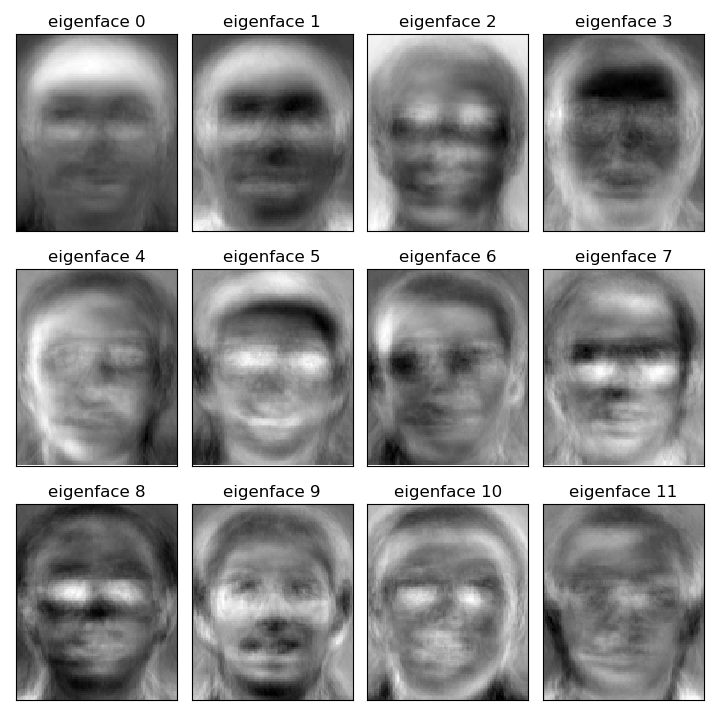
\includegraphics[width=0.4\textwidth]{eigenface.png}\
	  \caption{前11个特征脸}
	  \label{fig:oscil}
	\end{figure}


部分分类结果如下:

  \begin{figure}[H]
	  \centering
	  \label{fig:Per6A}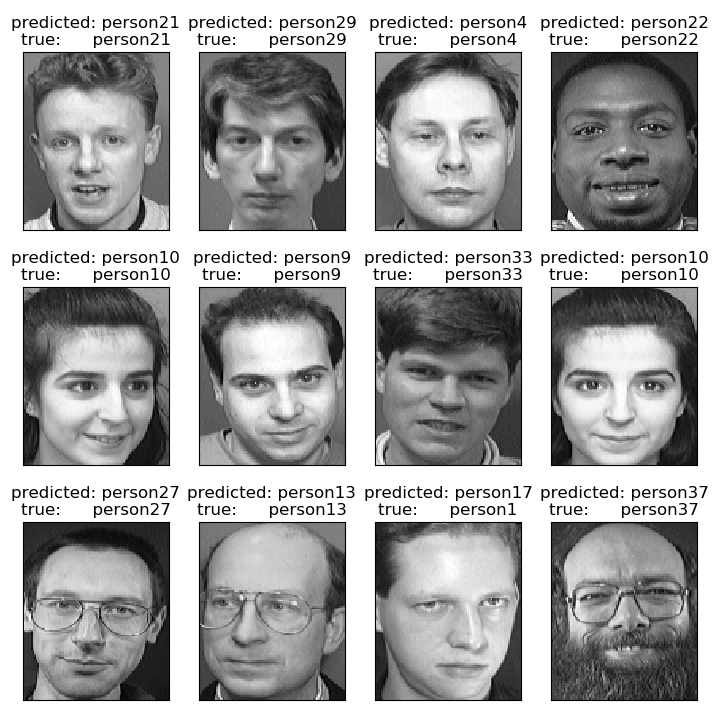
\includegraphics[width=0.8\textwidth]{precision.png}\
	  \caption{识别精确度}
	  \label{fig:oscil}
	\end{figure}

可以看出,该方法对于2D图像的人脸识别看可以达到较高的精度,图中仅有第三行第三列的人脸识别错误。

\newpage
\section{结论与讨论}
实验的目的是通过使用代码,了解如何使用机器学习方法实现人脸识别,熟悉相关的编程环境以及调用方式。底层的算法实现并不是本实验的要求。\vspace{3mm}

本文通过使用Sci-kit learn python库实现了人脸识别,尽管没有从最底层的代码进行实现,但是经过实验实现了三种降维算法的应用。通过实际的实验,对于特征脸的意义通过可视化有了更加直观的认识。对于算法原理也有了更深刻的认识。如果之后有时间,会花更多时间,从底层代码完成多种机器学习算法,而不是单纯调库。\vspace{3mm}

报告写作过程中参考了周志华《机器学习》,以及《Hands on machine learning with sci-kit learn》。代码demo部分来源于scikit-learn网站。\vspace{3mm}

最后感谢李教授这学期的教学,只是有些可惜课时太少,很希望未来机器学习这门课可以调整成全周的课程,顺颂时祺。\vspace{3mm}

\newpage
\section{附录}
实验使用的源代码如下.  \vspace{5mm}
	\lstinputlisting{face_recognition.py}
	\vspace{3mm}




\end{document} % DONE WITH DOCUMENT!





%%%%%%%%%%%%%%%%%%%%%%%%%%%%%%
\newpage
\section{Experiment Data}
This section will consist of the important code blocks which were changed in order to meet the requirements of the lab.  \vspace{5mm}
	\lstinputlisting{code.c}
	\vspace{3mm}



% IF YOU'D RATHER TYPE THE CODE, OR HAVE A SMALLER BLOCK OF CODE, USE THIS:
%\begin{lstlisting}
%if(something)
%	do this
%else
%	do this
%\end{lstlisting}

%% THIS IS FROM A DIFFERENT CLASS, BUT DEMONSTRATES MATH MODE WELL
%%%%%%%%%%%%%%%%%%%%%%%%%%%%%%
\subsection{Formulas and Overall Descriptions Used}
This part of the laboratory was done for \href{http://www.byui.edu/catalog/2004-2005/class.asp1075.htm}{Feedback Control}.  Most of this laboratory's calculations were completed and compiled by the folks at Quanser (the manufacturer of the inverted pendulum) and will give the lab a good starting place.  Below are the state equation and gain values used initially in the lab:
	\[
	\begin{bmatrix}
	\dot{\alpha} \\
	\ddot{\alpha} \\
	\dot{\theta} \\
	\ddot{\theta} \\
	\end{bmatrix}
	=
	\begin{bmatrix}
	0 & 1 & 0 & 0 \\
	81.7 & 0 & 0 & -13.9 \\
	0 & 0 & 0 & 1 \\
	39.7 & 0 & 0 & -14.4 \\
	\end{bmatrix}
	\begin{bmatrix}
	\alpha \\
	\dot{\alpha} \\
	\theta \\
	\dot{\theta} \\
	\end{bmatrix}
	+
	\begin{bmatrix}
	0 \\
	24.5 \\
	0 \\
	25.4 \\
	\end{bmatrix}
	V
	\]

	\[
	K  =
	\begin{bmatrix}
	21 & 2.8 & -2.2 & -2.0 \\
	\end{bmatrix}
	\]

Other values, such as the $\frac{\mbox{Volts}}{\mbox{Degree}}$ and $\frac{\mbox{Degrees}}{\mbox{Volt}}$ were obtained by first determining the max angle of the pendulum on both extreme sides.

Using the max angles from above, these values were determined:
	\[
	\begin{array}{l l}
		\alpha = 0.062 \frac{\mbox{Volts}}{\mbox{Degree}} \\ \\
		\alpha = 15.105 \frac{\mbox{Degrees}}{\mbox{Volt}} \\
	\end{array}
	\]

I would also like to add that in order to calibrate $\alpha$ to get a perfect vertical $= 0$, a value of $0.09$ needed to be added.  The same applies to $\theta$ where $0.322$ needs to be added.

%%%%%%%%%%%%%%%%%%%%%%%%%%%%%%
\subsection{DC Motor Transfer Function and Parameters}

Definitions:
	\begin{align*}
		\theta(t) =  Angular Position \\
		\dot{\theta}(t) =  Angular Velocity \\
		\triangle t = t_{10\%} - t_{90\%} \\
		90\% = e^{-t_{10\%}/\tau} \\
		10\% = e^{-t_{90\%}/\tau} \\
	\end{align*}

The Math:
	\begin{align*}
		\frac{s\theta(s)}{V_{a}(s)} = \frac{K}{s+P} \\
		\mbox{Let}\ V_{a}(s) = \frac{V_{0}}{s} \\  % If you'd like to have a space following any command, add "\" to the end as shown here.
		s\theta(s) = \frac{KV_{0}}{(S+P)S} = \frac{KV_{0}}{\frac{P}{S}} - \frac{\frac{KV_{0}}{P}}{s+P} \\
		L^{-1} \Rightarrow \dot{\theta}(t) = \frac{KV_{0}}{P}(1-e^{-t/(1/P)}) \\
		\dot{\theta}(t) = (\dot{\theta}_{i} - \dot{\theta}_{f})e^{-pt} + \dot{\theta}_{f} \\
	\end{align*}

Final equations:
	\begin{align}
		\label{thetadot}\dot{\theta}_{f} = \frac{KV_{0}}{P} \\
		\label{equ:tau}\frac{1}{P} = \tau = \frac{\triangle t}{ln(9)}
	\end{align}

Graphically (Refer to Equation \ref{thetadot} and Equation \ref{equ:tau}) :
	% Drawn and exported to png using Inkscape.
	\begin{figure}[h]
		\begin{center}
			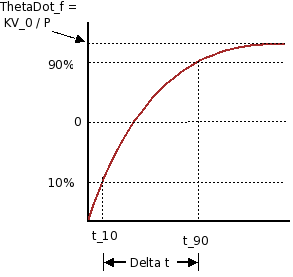
\includegraphics[width=0.33\textwidth]{graph.png}
		\end{center}
	\label{graph}
	\end{figure}

% AGAIN, ANOTHER EXAMPLE FROM A DIFFERENT CLASS WHICH DEMONSTRasdATES KMAPS AND TABLES NICELY.
\newpage % I added this after viewing the completed pdf and decided to make this cosmetic change
This section consists of tables and reductions which were used in this laboratory exercise.

% This table was generated using the Calc2LaTeX macro which I mentioned earlier.
% You'll need OpenOffice installed and you'll have to download the macro online.
% If you're interested, I have a guide on how to set this up and use it on my
% blog.  http://www.derekhildreth.com/blog  Search for "LaTeX".  You'll find it.
	\begin{table}[htbp]
	\begin{center}
		\begin{tabular}{|ccc|cc|}
			\hline
			\textbf{PS} & \textbf{D} & \textbf{N} & \textbf{NS} & \textbf{P} \\ \hline
			\$0.00 & 0 & 0 & \$0.00 & 0 \\
			 & 0 & 1 & \$0.05 & 0 \\
			 & 1 & 0 & \$0.10 & 0 \\
			 & 1 & 1 & -- & -- \\ \hline
			\$0.05 & 0 & 0 & \$0.05 & 0 \\
			 & 0 & 1 & \$0.10 & 0 \\
			 & 1 & 0 & \$0.15 & 0 \\
			 & 1 & 1 & -- & -- \\ \hline
			\$0.10 & 0 & 0 & \$0.10 & 0 \\
			 & 0 & 1 & \$0.15 & 0 \\
			 & 1 & 0 & \$0.15 & 0 \\
			 & 1 & 1 & -- & -- \\ \hline
			\$0.15 & -- & -- & \$0.15 & 1 \\ \hline
			\end{tabular}
	\end{center}
	\caption{Symbolic Transition Table}
	\label{symbolic}
	\end{table}

	\begin{table}[H]
		\centering
		\subfloat[D1 = $Q_{1}$+D+$Q_{0}$N] % Caption
			{
				\karnaughmap{4}{D1:}{ {$Q_{1}$} {$Q_{0}$} {D} {N} }{001X011X111X111X}{}  % See the included kvdoc.pdf file for more details
			} \hspace{10mm} % seperate them a bit
		\subfloat[D0 = $\Bar{Q_{0}}$N + $Q_{0}\Bar{N}$ + $Q_{1}$N + $Q_{1}$D] % Caption
			{
				\karnaughmap{4}{D0:}{ {$Q_{1}$} {$Q_{0}$} {D} {N} }{010X101X011X111X}{}
			}
	  \caption{Karnaugh maps and the simplified results of the logic.}
	  \label{fig:kmaps}
	\end{table}


%%%%%%%%%%%%%%%%%%%%%%%%%%%%%%
%%%%%%%%%%%%%%%%%%%%%%%%%%%%%%
\newpage
\section{Discussion \& Conclusion}
The goal of this lab was to re-design the LED/Switch system to include a hardware timer.  By pressing eight different combinations of the three buttons, the LEDs on the board were to act in different ways using these timers. There was not a Q\&A requirement for this lab. \vspace{3mm} % I use this to seperate the paragraphs a bit.

I was able to accomplish the requirements of the lab by utilizing the \texttt{IntMgrTimerExample.c} project found within the analog devices example programs folder (and mentioned in the class lecture).  There were some stumbling blocks to overcome.  The most difficult for myself was actually getting the period of the LEDs just right.  I was able to get it very close to the 333.3\ms, 666.7\ms, and 1\s periods, but not exactly.  My first method of getting these periods right was to take the clock speed in \MHz, find the period by taking the inverse of the clock speed, and then solving for the value in hex that was needed to get the right period.  This didn't yeild very accurate results at all, and so I then went through a trial and error session until I got a value of 1.1\ms.  I used this value in hex to calculate the other periods.  The results of this method can be seen in Figure \ref{fig:oscil} above in the schematics section. \vspace{3mm}

Another observation I would like to point out is that I put all of my logic within the interrupts themselves.  I feel that this was a hacked way of doing the lab to save time and that it's probably not the best programming method.  After I was completed with my lab, I viewed other students solutions and they just seemed more elegant.  Interestingly enough, the other students weren't incredibly happy with their solution either.  If I were to go back and do this lab again, I would invest more time in both understanding how to utilze the interrupts as well as find a more elegant solution to blink the lights. \vspace{3mm}

All in all, this laboratory gave me an insight on how interrupts work and I hope to be able to apply them to following labs\ldots


\end{document} % DONE WITH DOCUMENT!


%%%%%%%%%%
PERSONAL FAVORITE LAB WRITE-UP STRUCTURE
%%%%%%%%%%
\section{Introduction}
	% No Text Here
	\subsection{Purpose}
		% Lab objective
	\subsection{Equipment}
		% Any and all equipment used (specific!)
	\subsection{Procedure}
		% Overview of the procedure taken (not-so-specific!)
\newpage
\section{Schematic Diagrams}
	% Any schematics, screenshots, block
   % diagrams used.  Possibly photos or
	% images could go here as well.
\newpage
\section{Experiment Data}
	% Depending on lab, program code would be
	% included here without the Estimated and
	% Actual Results.
	\subsection{Estimated Results}
		% Calculated. What it should be.
	\subsection{Actual Results}
		% Measured.  What it actually was.
\newpage
\section{Discussion \& Conclusion}
	% 3 Paragraphs:
		% Restate the objective of the lab
		% Discuss personal trials, errors, and difficulties
		% Conclude the lab


%%%%%%%%%%%%%%%%
COMMON COMMANDS:
%%%%%%%%%%%%%%%%
% IMAGES
begin{figure}[H]
   \begin{center}
      \includegraphics[width=0.6\textwidth]{RTL_SCHEM.png}
   \end{center}
\caption{A screenshot of the RTL Schematics produced from the Verilog code.}
\label{RTL}
\end{figure}

% SUBFIGURES IMAGES
\begin{figure}[H]
  \centering
  \subfloat[LED4 Period]{\label{fig:Per4}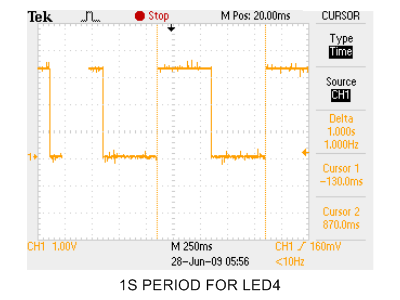
\includegraphics[width=0.4\textwidth]{period_led4.png}} \\
  \subfloat[LED5 Period]{\label{fig:Per5}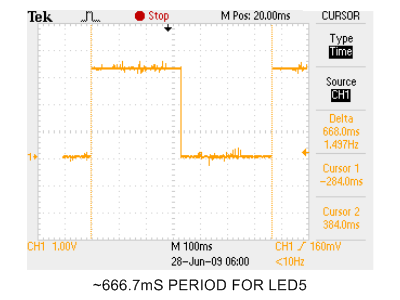
\includegraphics[width=0.4\textwidth]{period_led5.png}}
  \subfloat[LED6 Period]{\label{fig:Per6}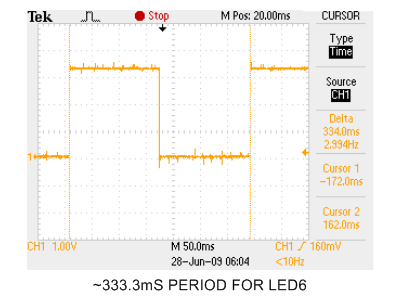
\includegraphics[width=0.4\textwidth]{period_led6.png}}
  \caption{Period of LED blink rate captured by osciliscope.}
  \label{fig:oscil}
\end{figure}

% INSERT SOURCE CODE
\lstset{language=Verilog, tabsize=3, backgroundcolor=\color{mygrey}, basicstyle=\small, commentstyle=\color{BrickRed}}
\lstinputlisting{MODULE.v}

% TEXT TABLE
\begin{table}
\begin{center}
\begin{tabular}{|l|c|c|l|}
	x & x & x & x \\ \hline
	x & x & x & x \\
	x & x & x & x \\ \hline
\end{tabular}
\caption{Caption}
\label{label}
\end{center}
\end{table}

% MATHMATICAL ENVIRONMENT
$ 8 = 2 \times 4 $

% CENTERED FORMULA
\[  \]

% NUMBERED EQUATION
\begin{equation}

\end{equation}

% ARRAY OF EQUATIONS (The splat supresses the numbering)
\begin{align*}

\end{align*}

% NUMBERED ARRAY OF EQUATIONS
\begin{align}

\end{align}

% ACCENTS
\dot{x} % dot
\ddot{x} % double dot
\bar{x} % bar
\tilde{x} % tilde
\vec{x} % vector
\hat{x} % hat
\acute{x} % acute
\grave{x} % grave
\breve{x} % breve
\check{x} % dot (cowboy hat)

% FONTS
\mathrm{text} % roman
\mathsf{text} % sans serif
\mathtt{text} % Typewriter
\mathbb{text} % Blackboard bold
\mathcal{text} % Caligraphy
\mathfrak{text} % Fraktur

\textbf{text} % bold
\textit{text} % italic
\textsl{text} % slanted
\textsc{text} % small caps
\texttt{text} % typewriter
\underline{text} % underline
\emph{text} % emphasized

\begin{tiny}text\end{tiny} % Tiny
\begin{scriptsize}text\end{scriptsize} % Script Size
\begin{footnotesize}text\end{footnotesize} % Footnote Size
\begin{small}text\end{small} % Small
\begin{normalsize}text\end{normalsize} % Normal Size
\begin{large}text\end{large} % Large
\begin{Large}text\end{Large} % Larger
\begin{LARGE}text\end{LARGE} % Very Large
\begin{huge}text\end{huge}   % Huge
\begin{Huge}text\end{Huge}   % Very Huge


% GENERATE TABLE OF CONTENTS AND/OR TABLE OF FIGURES
% These seem to have some issues with the "revtex4" document class.  To use, change
% the very first line of this document to "article" like this:
% \documentclass[aps,letterpaper,10pt]{article}
\tableofcontents
\listoffigures
\listoftables

% INCLUDE A HYPERLINK OR URL
\url{http://www.derekhildreth.com}
\href{http://www.derekhildreth.com}{Derek Hildreth's Website}

% FOR MORE, REFER TO THE "LINUX CHEAT SHEET.PDF" FILE INCLUDED!
